\chapter{TINJAUAN PUSTAKA}

% Ubah konten-konten berikut sesuai dengan isi dari tinjauan pustaka
\section{Hasil penelitian terdahulu}
Pada subbab berikut akan dijabarkan mengenai penelitian terdahulu yang mengambil topik yang sama ataupun beririsan sebagai referensi, serta dasar pengembangan dan inovasi pada tugas akhir ini.
\subsection{Deep Learning-Based Object Detection, Localisation and Tracking
for Smart Wheelchair Healthcare Mobility} Penelitian dengan judul "Deep Learning-Based Object Detection, Localisation and Tracking for Smart Wheelchair Healthcare Mobility" yang diteliti oleh Lecrosnier, L., Khemmar, R., Ragot, N., et al.
Penelitian ini bertujuan untuk mengembangkan sistem bantuan pengemudi tingkat lanjut untuk mobil. Kursi roda elektrik pintar untuk meningkatkan kemandirian penyandang disabilitas. Penelitian ini berfokus pada deteksi objek dalam ruangan, lokalisasi, dan pelacakan.
Kursi roda, terutama pintu dan gagang pintu.
Tujuan utama dari penelitian ini adalah untuk meningkatkan fungsionalitas kursi roda otonom. Ini memungkinkan untuk mendeteksi objek-objek ini di sekitar secara akurat. langkah pertama Penelitian ini bertujuan untuk mengadaptasi algoritma deteksi objek YOLOv3 dengan kasus kami. Penggunaannya. Selain itu, penelitian ini menggunakan kamera Intel RealSense untuk Metode estimasi kedalaman. Terakhir, sebagai langkah ketiga dan terakhir, penelitian ini Kami menggunakan pendekatan pelacakan objek 3D berdasarkan algoritma SORT. \cite{Lecrosnier2021}

\subsection{Deteksi Fitur Huruf Sistem Isyarat Bahasa Indonesia menggunakan Metode Chain Code}
Berdasarkan penelitian yang dilakukan oleh Afifah Nur dan Hendro Nugroho berhasil dalam melakukan deteksi SIBI dengan menggunakan 119 data training dan 52 data testing dengan akurasi terbesar yakni 96.961\% dan akurasi terendah yaitu 84.762\%. Penggunaan metode \emph{Chain Code}, \emph{Chain Code} adalah teknik representasi kontur atau bentuk dalam citra digital menggunakan urutan arah tertentu. Teknik ini digunakan dalam pemrosesan citra untuk menggambarkan tepi objek secara efisien dan kompak. Chain code merepresentasikan kontur dengan merekam langkah-langkah yang mengikuti batas objek berdasarkan arah relatif antara titik-titik tetangga. \cite{Afifah2022}

\subsection{Pendeteksian Bahasa Isyarat Indonesia Secara \emph{Real-Time} menggunakan \emph{Long Short-Term Memory} (LSTM)}
Penelitian yang dilakukan oleh Husna Moetia Putri, Fadlisyah, dan Wahyu Fuadi berhasil
melakukan pendeteksian bahasa isyarat Indonesia secara real-time menggunakan arsitektur Long
Short-Term Memory (LSTM) dan MediaPipe Holistic. Pada pengujian menggunakan 10 kosakata
isyarat BISINDO didapat evaluasi akurasi sebesar 92% dengan menggunakan bidirectional
layer LSTM, epoch 1000, hidden layer 64, batch size 32. Sedangkan, pada pengujian meng-
gunakan 30 kosakata isyarat BISINDO didapat evaluasi akurasi sebesar 65% dengan menggu-
nakan 2 buah layer LSTM epoch 500, hidden layer 64, batch size 64. 

\section{Teori Dasar}
\subsection{Gestur}
Gestur adalah gerakan tubuh, terutama tangan, lengan, kepala, atau bagian tubuh lainnya, yang digunakan untuk menyampaikan informasi, ekspresi, atau niat tertentu, baik secara sengaja maupun tidak sengaja. Dalam konteks komunikasi non-verbal, gestur berfungsi untuk melengkapi atau menggantikan kata-kata, seperti melambaikan tangan untuk menyapa atau menganggukkan kepala sebagai tanda persetujuan. Dalam bidang teknologi, gesture sering digunakan sebagai metode interaksi manusia dengan komputer (HCI), di mana gerakan tubuh menjadi input untuk mengontrol sistem, misalnya melalui pengenalan gerakan tangan menggunakan sensor atau kamera. Gesture juga memiliki peran penting dalam psikologi dan studi kognitif, karena dapat mencerminkan proses berpikir dan emosi seseorang. Dalam penelitian berbasis analisis visual, gesture sering diidentifikasi untuk memahami pola gerakan atau mengembangkan teknologi interaktif. Dengan perannya yang luas, gesture menjadi elemen penting dalam berbagai bidang penelitian, terutama yang berfokus pada komunikasi, perilaku manusia, atau interaksi teknologi.
\subsection{Sistem Isyarat Bahasa Indonesia (SIBI)}
Sistem SIBI (Sistem Isyarat Bahasa Indonesia) adalah suatu sistem komunikasi yang menggunakan gerakan tangan, ekspresi wajah, dan posisi tubuh untuk menyampaikan pesan dalam bentuk bahasa. SIBI dirancang sebagai representasi visual dari Bahasa Indonesia yang ditujukan untuk membantu komunikasi dengan atau di antara penyandang tunarungu. Sistem ini memadukan simbol-simbol isyarat yang sesuai dengan tata bahasa Bahasa Indonesia, sehingga setiap kata dan kalimat diisyaratkan berdasarkan urutan gramatikal Bahasa Indonesia yang baku.\begin{figure} [H] \centering
  % Nama dari file gambar yang diinputkan
  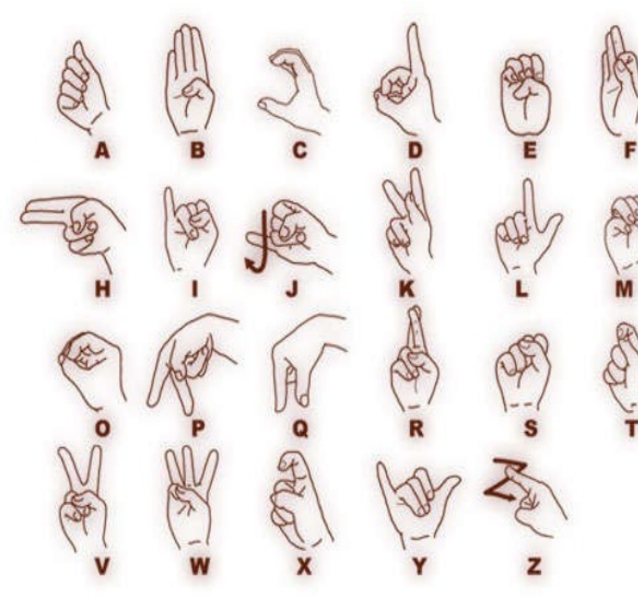
\includegraphics[scale=0.7]{gambar/SIBI Gesture.png}
  % Keterangan gambar yang diinputkan
  \caption{Gesture tangan untuk SIBI }
  % Label referensi dari gambar yang diinputkan
  \label{fig:Sibi}
\end{figure}
\subsection{Object Detection}
\emph{Object Detection} adalah teknik visi komputer yang membantu mengidentifikasi dan menemukan objek dalam gambar dan video. Dengan bentuk identifikasi dan pelokalan ini, deteksi objek dapat digunakan untuk menghitung jumlah item dalam sebuah skenario, menemukan dan mengidentifikasi mereka dengan tepat, serta memberikan nama. Pendeteksian objek tetap menjadi salah satu aspek paling mendasar dan menantang dalam aplikasi visi komputer dan pemahaman citra. Kemajuan signifikan dalam deteksi objek telah dicapai melalui representasi objek yang lebih baik dan penggunaan model jaringan saraf dalam (deep neural networks). Metode deteksi objek telah berkembang pesat dengan penggunaan jaringan saraf konvolusional (CNN) dan algoritme khusus seperti YOLO (You Only Look Once) dan SSD (Single Shot Multibox Detector).
Selain kerangka YOLO, kemajuan juga telah dicapai di bidang deteksi objek dan pemrosesan gambar.Memperluas beberapa metode terkenal lainnya. Teknologi seperti R-CNN (Konvolusi Berbasis Wilayah), (Neural Networks nasional) dan penerusnya Fast R-CNN dan Faster R-CNN.
Ini memainkan peran penting dalam meningkatkan akurasi deteksi objek. Metode ini bergantung pada dua proses Tahap tersebut melakukan pencarian selektif untuk menghasilkan proposal wilayah dan menghasilkan jaringan saraf konvolusional.Klasifikasi dan penyempurnaan area ini. Pendekatan penting lainnya adalah Single-Shot MultiBox Detector (SSD), yang mirip dengan YOLO dalam mengutamakan kecepatan dan efisiensi dengan menghilangkan kebutuhan akan langkah proposal wilayah secara terpisah. Di sisi lain, metode seperti Mask R-CNN telah meningkatkan kemampuan deteksi objek hingga mencakup segmentasi instans, memungkinkan pelokalan objek yang lebih presisi hingga tingkat piksel. Perkembangan ini, bersama metode lainnya seperti RetinaNet dan EfficientDet, secara kolektif telah memperkaya keragaman algoritma deteksi objek. Setiap algoritma ini menawarkan keseimbangan yang berbeda antara kecepatan, akurasi, dan tingkat kompleksitas, yang dirancang untuk memenuhi berbagai kebutuhan aplikasi dan batasan komputasi.

\subsection{Convolutional Neural Network (CNN)}

Convolutional Neural Network (CNN) adalah jenis lapisan \emph{deep learning} yang dirancang khusus untuk memproses data dalam bentuk grid seperti gambar. CNN merupakan lapisan dasar yang digunakan dalam membangun arsitektur YOLO. Dimana dalam penggunaannya CNN memiliki beberapa lapisan (\emph{layers}) yang secara hierarkis mengekstrak fitur dari data masukan. Berikut adalah penjelasan mengenai komponen utama dari CNN:

\subsubsection{Lapisan Konvolusi (\emph{Convolutional Layer})}

Lapisan konvolusi adalah inti dari CNN. Pada lapisan ini, filter (\emph{kernels}) diterapkan pada input untuk menghasilkan peta fitur (\emph{feature map}). Filter ini bergerak melintasi input dengan operasi konvolusi, menangkap pola lokal seperti tepi, tekstur, dan bentuk. Setiap filter mempelajari fitur yang berbeda dari data. berikut merupakan rumus untuk operasi konvolusi dalam konteks matematika dan pemrosesan sinyal.

\begin{equation}
    (f * g)(t) = \int_{-\infty}^{\infty} f(\tau)g(t - \tau) \, d\tau
\end{equation}

\subsubsection{Lapisan Aktivasi (\emph{Activation Layer})}

Lapisan aktivasi memperkenalkan non-linearitas ke dalam model, memungkinkan jaringan untuk mempelajari hubungan yang kompleks. Fungsi aktivasi yang umum digunakan adalah ReLU (\emph{Rectified Linear Unit}), yang mendefinisikan \( f(x) = \max(0, x) \). Fungsi ini menggantikan nilai negatif dalam peta fitur dengan nol.

\subsubsection{Lapisan Pooling (\emph{Pooling Layer})}

Lapisan pooling mengurangi dimensi spasial dari peta fitur, mengurangi jumlah parameter dan komputasi dalam jaringan. Tipe pooling yang sering digunakan adalah \emph{max pooling}, yang memilih nilai maksimum dalam setiap jendela pooling. Pooling membantu dalam membuat deteksi fitur lebih robust terhadap perubahan posisi dan skala.

\subsubsection{Lapisan Fully Connected (\emph{Fully Connected Layer})}

Pada lapisan fully connected, setiap neuron terhubung dengan semua neuron di lapisan sebelumnya. Lapisan ini biasanya terletak di akhir jaringan dan digunakan untuk menggabungkan fitur-fitur yang telah diekstraksi menjadi prediksi akhir. 

\subsubsection{Lapisan Output (\emph{Output Layer})}
Lapisan output menghasilkan prediksi akhir dari model. Dalam konteks deteksi objek, lapisan ini dapat menghasilkan hasil kelas objek yang terdeteksi. Fungsi aktivasi softmax sering digunakan untuk klasifikasi multi-kelas, sedangkan fungsi sigmoid digunakan untuk deteksi objek dengan beberapa kelas.


\subsection{YOLO(You Look Only Once)}
YOLO (You Only Look Once) adalah salah satu algoritma deteksi objek dalam visi komputer yang dirancang untuk mendeteksi dan mengidentifikasi objek dalam gambar atau video secara cepat dan akurat. YOLO bekerja dengan cara menganalisis gambar secara keseluruhan dalam satu kali pemrosesan (hence "You Only Look Once"), berbeda dengan metode lainnya yang sering memproses gambar secara bertahap atau melalui beberapa langkah, seperti mengidentifikasi wilayah objek terlebih dahulu baru kemudian mengklasifikasikan objek tersebut.

Pada dasarnya, YOLO membagi gambar menjadi grid dan, untuk setiap grid, memprediksi berbagai kotak pembatas (bounding boxes) dan kemungkinan kelas objek yang ada di dalamnya. Hal ini memungkinkan YOLO untuk mendeteksi beberapa objek dalam satu gambar secara bersamaan dalam satu waktu pemrosesan, sehingga sangat efisien dalam hal kecepatan.

\newpage
\subsection{YOLOv11}
YOLOv11 merupakan iterasi terbaru dalam seri pengembangan YOLO yang memperkenalkan peningkatan arsitektur baru, termasuk mekanisme perhatian yang lebih baik, lapisan ekstraksi fitur yang lebih dalam, dan paradigma deteksi tanpa jangkar (anchor-free). Inovasi-inovasi ini dirancang untuk mengatasi tantangan dalam mendeteksi kendaraan yang lebih kecil, tersembunyi, atau bergerak cepat, sambil mempertahankan kemampuan inferensi waktu nyata. YOLOv11 juga dioptimalkan untuk percepatan perangkat keras, membuatnya lebih kompatibel dengan perangkat tepi yang digunakan dalam aplikasi kritis seperti deteksi emosi dan sistem transportasi cerdas.
Peningkatan dalam YOLOv11, khususnya dengan pengenalan deteksi tanpa jangkar dan mekanisme perhatian yang lebih baik, menandakan langkah maju dalam pengembangan sistem deteksi kendaraan yang kuat dan dapat diskalakan.
Penggunaan YOLOv11 ini bertujuan untuk mengevaluasi kinerja YOLOv11 dalam konteks deteksi objek pada kursi roda, dengan fokus pada kemampuannya untuk menangani skenario deteksi yang kompleks dan waktu nyata. Hasil evaluasi YOLOv11 dibandingkan dengan pendahulunya, YOLOv8, menggunakan metrik utama seperti presisi, recall, dan mean average precision (mAP).
\begin{figure} [H] \centering
  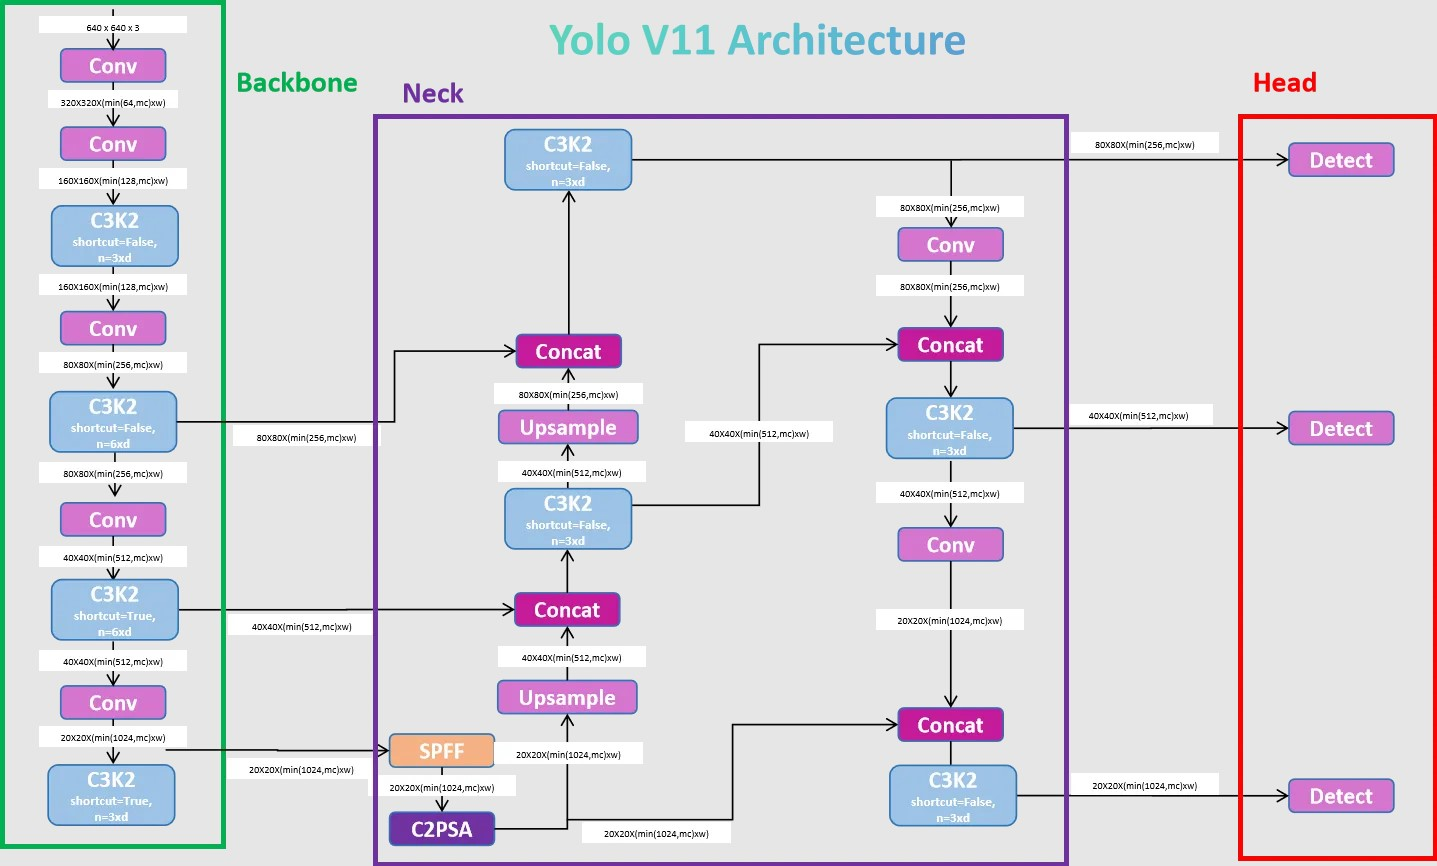
\includegraphics[width=\textwidth]{gambar/Arsitektur YOLOv11.jpg}
  \caption{Arsitektur dari YOLOv11 }
  \label{fig:YOLOv11}
\end{figure}
\subsection{LSTM(Long Short-Term Memory)}
\emph{Long Short-Term Memory} (LSTM) (LSTM) adalah bentuk RNN yang sering digunakan untuk menghindari masalah Penumpukan dengan gradasi, ketergantungan jangka panjang pada memproses atau membuat prediksi ke data deret waktu. RNN cenderung memiliki penumpukan pada gradien yang menyebabkan nilai gradien saling bertabrakan sehingga terdapat nilai gradien yang tidak jelas dan dapat menghilangkan nilai akumulasinya sehingga diperlukan LSTM untuk menghindari hal tersebut terjadi\cite{Cholissodin2019}.

Menurut Sepp Hochreiter dan Jurgen Schmidhuber, model LSTM terbentuk dari berbagai rangkaian sel memori yang dapat menggantikan sel neuron pada hidden layer dari RNN. Model LSTM dapat menyaring data atau informasi memlalu struktur gates untuk dapat mempertahankan informasi yang berhubungan dan mengubah keadaan dari sel memori. Struktur gerbang tersebut mencakup input gate, forgate gate, dan output gate\cite{Larasati2021}. 
\begin{figure} [H] \centering
  % Nama dari file gambar yang diinputkan
  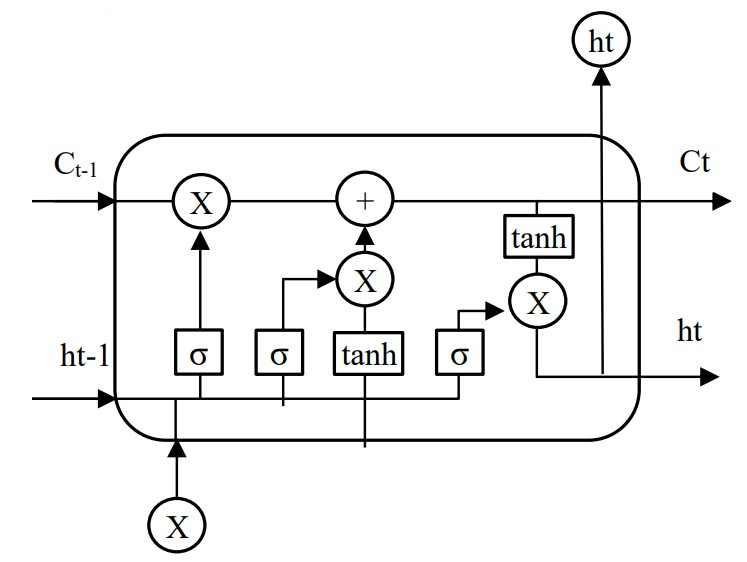
\includegraphics[scale=0.55]{gambar/LSTM.jpg}
  % Keterangan gambar yang diinputkan
  \caption{Arsitektur dari LSTM }
  % Label referensi dari gambar yang diinputkan
  \label{fig:Arsitektur LSTM }
\end{figure}
LSTM terdiri dari rangkaian sel memori yang unik dan model LSTM menyaring informasi
melalui struktur gerbang. Pada LSTM terdapat 3 gerbang atau Gates Unit dan 1 Cell states, yaitu input gates, forget gate, output gates, dan cell states. Persamaan dari setiap gate sebagai berikut:
\subsubsection{Input gates}
\emph{Input gate}menerima informasi berupa \emph{hidden state} yang berasal dari sel sebelumnya dan informasi baru yang berasal dari masukan saat ini, dan informasi tersebut digabungkan dan diproses menggunakan fungsi sigmoid dan tanh. Hasil dari fungsi sigmoid mengubah nilai dari 0 menjadi 1 dan menentukan informasi mana yang diperbarui. Nilai yang mendekati 0 berarti informasi tersebut tidak penting, dan nilai yang mendekati 1 berarti informasi tersebut penting. Hasil fungsi Tanh berupa nilai antara -1 dan 1 digunakan untuk membantu sel mempelajari informasi dengan lebih baik.
 Persamaan dari \emph{input gate} adalah sebagai berikut:
\begin{equation}
  \label{eq:InputGate}
  i_t = \sigma(W_i \times X_i + U_i \times h_{t-1} + b_i)
\end{equation}
Dalam persamaan ini, \( i_t \) mewakili nilai dari input gate, yang dihitung dengan menggunakan fungsi aktivasi sigmoid \( \sigma \), yang menghasilkan output antara 0 dan 1. Ini memungkinkan model untuk mengontrol secara dinamis seberapa banyak informasi dari input saat ini (\( X_i \)) dan keadaan tersembunyi sebelumnya (\( h_{t-1} \)) yang akan diterima dan disimpan dalam memori. Faktor \( W_i \) dan \( U_i \) adalah bobot yang masing-masing terkait dengan input \( X_i \) dan keadaan tersembunyi sebelumnya \( h_{t-1} \), sementara \( b_i \) adalah bias yang membantu menyesuaikan perhitungan tersebut.
\subsubsection{Forget gates}
\emph{Forget gates} memutuskan informasi apa yang akan disimpan atau dibuang. Forget gate menerima informasi berupa \emph{hidden state} yang berasal dari sel sebelumnya dan informasi baru yang berasal dari \emph{input} saat ini. Informasi ini kemudian digabungkan dan diproses menggunakan fungsi sigmoid sehingga menghasilkan hasil dalam bentuk 0 hingga  1. Semakin dekat hasil yang diperoleh ke 0, semakin banyak informasi yang dibuang, dan sebaliknya, semakin dekat hasil yang diperoleh ke 1, semakin banyak informasi yang disimpan. Persamaan dari \emph{forget gate} adalah sebagai berikut:
\begin{equation}
  \label{eq:ForgetGate}
  f_t = \sigma(W_f \times X_t + U_f \times h_{t-1} + b_f)
\end{equation}
Pada dasarnya, forget gate memeriksa data baru (\( X_t \)) dan informasi historis dari hidden state sebelumnya (\( h_{t-1} \)) untuk memutuskan seberapa besar kontribusi \( c_{t-1} \) yang akan diteruskan ke sel memori pada waktu \( t \). Ini adalah langkah penting dalam mengontrol ``memori jangka panjang'' pada LSTM, yang memungkinkan jaringan untuk menangani dependensi jangka panjang dalam data.

Jika nilai \( f_t \) mendekati 0, maka sebagian besar informasi dari memori sebelumnya akan dilupakan. Sebaliknya, jika \( f_t \) mendekati 1, informasi tersebut akan dipertahankan dalam memori selanjutnya. Ini membantu LSTM mengelola informasi yang relevan dan membuang informasi yang tidak berguna.
\subsubsection{Output gates}
\emph{Output gates} menentukan \emph{hidden state} yang dikirim ke sel berikutnya.\emph{Output gate} menerima informasi berupa \emph{hidden state} yang berasal dari sel sebelumnya, informasi baru yang berasal dari masukan saat ini, dan informasi tersebut digabungkan dan diproses dengan fungsi sigmoid. Status sel baru ditangani melalui fungsi tanh. Hasil fungsi Tanh dikalikan dengan hasil fungsi sigmoid untuk memperoleh informasi yang disimpan dalam keadaan tersembunyi baru. Status tersembunyi dan status sel baru ditransfer ke sel berikutnya. Berikut adalah persamaan dari \emph{output gate}:
\begin{equation}
  \label{eq:OutputGate}
  o_t = \sigma(W_o \times X_i + U_o \times h_{t-1} + b_o)
\end{equation}
Output gate pada LSTM mengontrol informasi yang akan diteruskan dari cell state \( c_t \) ke hidden state \( h_t \) dan akhirnya menjadi output model. Ini penting karena hidden state (\( h_t \)) membawa informasi yang diperlukan untuk prediksi pada langkah berikutnya, dan juga dapat digunakan sebagai output model dalam tugas-tugas seperti klasifikasi atau prediksi deret waktu.

Setelah output gate dihitung, informasi dari cell state \( c_t \) diubah dengan fungsi tanh (fungsi aktivasi hiperbolik tangen) untuk memastikan nilai berada dalam rentang yang sesuai sebelum diteruskan melalui output gate. Prosesnya adalah sebagai berikut:
\begin{equation}
  \label{eq:OutputGate dari LSTM}
  h_t = o_t \times \tanh(c_t)
\end{equation}
Di sini, \( \tanh(c_t) \) mengubah nilai cell state menjadi nilai yang lebih terkontrol sebelum dihasilkan sebagai output.
\subsection{Mediapipe}
MediaPipe adalah kerangka kerja yang dirancang oleh Google untuk dikembangkan.
Saluran pengenalan waktu nyata. MediaPipe memungkinkan pengembang untuk berintegrasi
Integrasikan berbagai jenis data sensor seperti video, audio, dan data lainnya ke dalam satu platform ini efisien dan dapat berjalan di berbagai perangkat mulai dari seluler hingga desktop.
Framework ini menggunakan konsep “grafik”, jadi setiap node dalam grafik Ini adalah "kalkulator" yang melakukan tugas-tugas tertentu seperti deteksi objek, pelacakan, dll. pose, atau segmentasi gambar. Masing-masing node ini dapat dikonfigurasi melalui GraphConfig.Salah satu penerapan MediaPipe yang paling dikenal adalah pada estimasi pose manusia menggunakan MediaPipe Pose. Metode ini menggabungkan estimasi pose 2D dengan model
humanoid yang lebih kompleks serta metode optimasi untuk mengestimasi sudut sendi pada
pose 3D. Metode ini terbukti efektif dalam mengatasi masalah ambiguitas kedalaman pada es-
timasi pose 3D dan dapat berjalan secara real-time bahkan pada perangkat tanpa GPU\cite{Lugaresi2019}.
\subsubsection{MediaPipe Pose}
MediaPipe Pose (MPP) adalah kerangka kerja sumber terbuka yang disediakan oleh Google.
Digunakan untuk mendapatkan perkiraan koordinat sendi manusia 2D dalam setiap bingkai gambar batang. MediaPipe Pose membangun saluran untuk memproses data kognitif dalam beberapa bagian untuk video menggunakan \emph{Machine Learning} (ML). Penerapan MPP
BlazePose mengekstrak 33 landmark 2D tubuh manusia seperti yang ditunjukkan.
Dapat dilihat pada Gambar 2.4. BlazePose adalah arsitektur pembelajaran mesin ringan yang memungkinkan kesamaan pekerjaan real-time di ponsel dan PC dengan inferensi CPU.Ketika menggunakan koordinat yang dinormalisasi untuk estimasi pose, rasio invers harus dikalikan dengan nilai piksel sumbu-y\cite{kim2023human}.
\begin{figure} [H] \centering
  % Nama dari file gambar yang diinputkan
  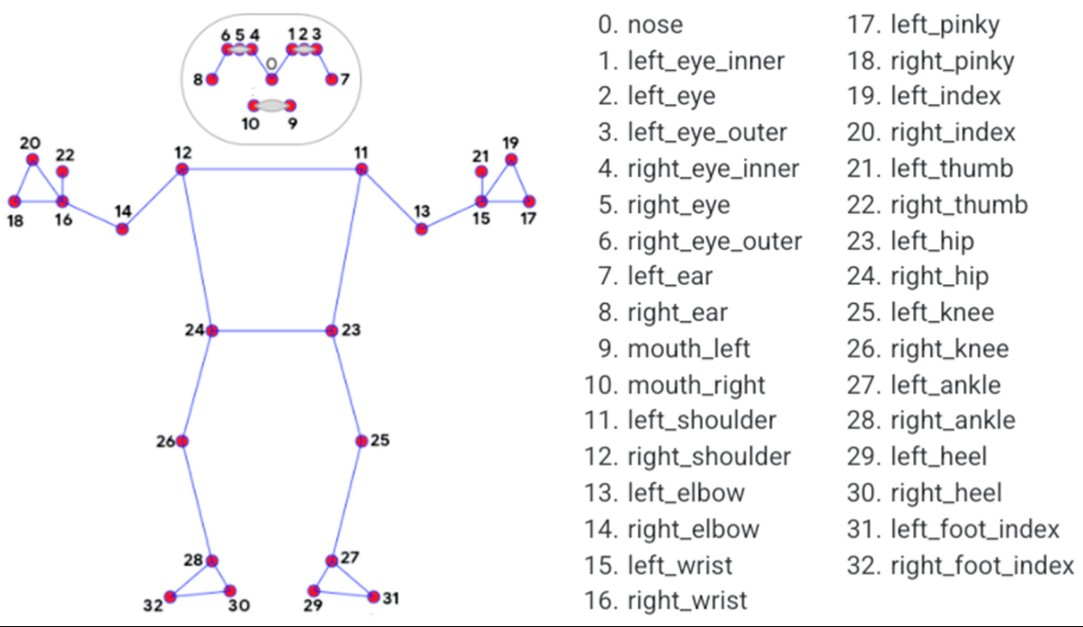
\includegraphics[scale=0.3]{gambar/mediapipepose.jpg}
  % Keterangan gambar yang diinputkan
  \caption{Pose MediaPipe }
  % Label referensi dari gambar yang diinputkan
  \label{fig:Pose MediaPipe }
\end{figure}

\subsection{Classification Performance}
\emph{Classification Performance} adalah sekumpulan metrik yang digunakan untuk mengevaluasi kinerja model klasifikasi. Metrik ini digunakan untuk menilai akurasi model, presisi, perolehan kembali, dan aspek lainnya. Ini sering digunakan untuk membandingkan model yang berbeda atau menyetel satu model untuk kinerja optimal. Metrik klasifikasi dapat dikelompokkan menjadi tiga kategori utama: Akurasi, sensitivitas, spesifisitas. Akurasi mengukur performa model secara keseluruhan dan biasanya merupakan metrik yang paling penting. Sensitivitas dan spesifisitas mengukur seberapa baik suatu model dapat membedakan kelas yang berbeda. Terakhir, metrik lain seperti skor AUC, skor F1, dan skor Kappa mengukur akurasi dan pengenalan model.  Dalam hal ini, confusion matrix merupakan salah satu perhitungan yang sering digunakan dalam kasus
pengklasifikasian.
\subsubsection{Confusion Matrix}
\emph{Confusion matrix} adalah salah satu pengukuran paling sederhana
Mencari tingkat nilai kebenaran dan keakuratan model. \emph{Confusion matrix}
merupakan tabel dua dimensi berisi data aktual dan prediksi, masing-masing dengan kelasnya. Data aktual ada di bagian kolom tabel dan data prediksi ada di bagian baris tabel. Gambar 2.5 merupakan representasi visual dari perhitungan confusion matrix. 
\begin{figure} [H] \centering
  % Nama dari file gambar yang diinputkan
  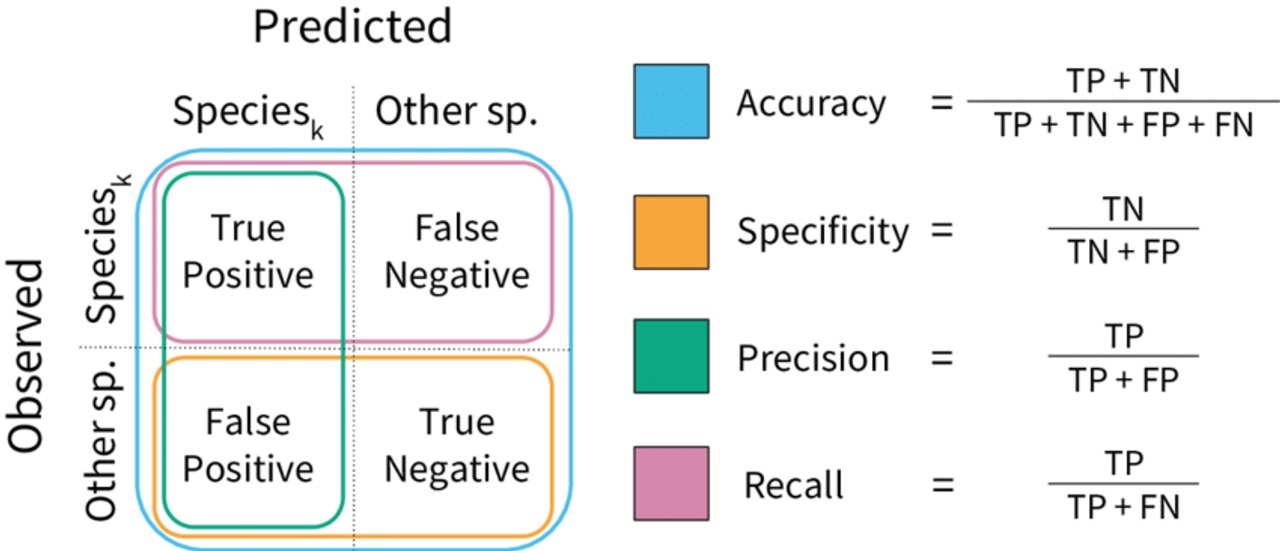
\includegraphics[scale=0.3]{gambar/confusionmatrix.jpg}
  % Keterangan gambar yang diinputkan
  \caption{Confusion Matrix }
  % Label referensi dari gambar yang diinputkan
  \label{fig:Confusion matrix }
\end{figure}

\subsection{Evaluation Matrix}
\emph{Evaluation Matrix} adalah cara untuk mengevaluasi sejumlah besar peringkat secara objektif. Pilihan untuk beberapa kriteria. Kriteria ini akan diprioritaskan sebelum evaluasi. Ini telah dibuat dengan lebih menekankan pada item yang paling penting.Terdapat dua tingkatan dalam \emph{evaluation matrix}. tingkat pertama ini bertindak sebagai filter di mana setiap opsi dievaluasi berdasarkan kriteria yang diperlukan pilihan-pilihan itu
yang memenuhi semua kriteria yang dipersyaratkan akan maju ke tingkat kedua dan dievaluasi kriteria prioritas. 

Metrik seperti akurasi, presisi, recall adalah kunci saat mengevaluasi seberapa efektif suatu model dalam mendeteksi dan mengidentifikasi objek. 
Lebih lanjut, analisis akurasi memberikan wawasan kuantitatif yang signifikan mengenai
kinerja algoritma deteksi objek, memberikan detail lebih lanjut mengenai kemampuan algo-
ritma dalam menghasilkan deteksi yang akurat. Mengenali kesalahan melalui metrik evaluasi
adalah langkah kritis dalam penelitian deteksi, seperti dalam kasus deteksi asap yang kami
teliti. Langkah ini memfasilitasi identifikasi dan pemahaman tentang potensi kesalahan dalamalgoritma, yang dapat membuka jalan untuk perbaikan dan peningkatan metode deteksi. Selanjutnya, metrik evaluasi juga mendukung pengoptimalan hiperparameter algoritma.
Dalam konteks penelitian ini, berbagai indikator evaluasi telah diterapkan, termasuk presisi, recall, dan Mean Average Precision (mAP). . Dengan menggabungkan metode evaluasi ini,Penelitian ini bertujuan untuk menyajikan analisis komprehensif terhadap kinerja algoritma deteksi objek yang sedang ditinjau.

\subsection{Intersection over Union(IoU)}
Intersection over Union adalah metrik populer untuk mengukur akurasi pelokalan dan menghitung kesalahan pelokalan dalam model deteksi objek. Ini menghitung jumlah tumpang tindih antara dua kotak pembatas—kotak pembatas yang diprediksi dan kotak pembatas kebenaran dasar. IoU adalah rasio perpotongan luas dua kotak dengan luas gabungannya. Kotak pembatas kebenaran dasar dan kotak pembatas yang diantisipasi keduanya mencakup area gabungan, yang merupakan penyebutnya.
\begin{figure} [H] \centering
  % Nama dari file gambar yang diinputkan
  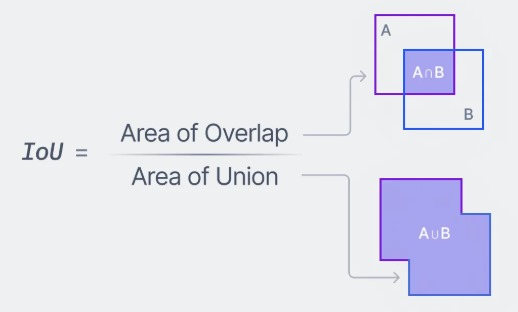
\includegraphics[scale=0.6]{gambar/IoU.jpg}
  % Keterangan gambar yang diinputkan
  \caption{Penggambaran dari IoU }
  % Label referensi dari gambar yang diinputkan
  \label{fig:Intersection over Union }
\end{figure}
IoU, atau Intersection over Union, merupakan metode penilaian yang mengukur efektivi-
tas model deteksi objek dengan membandingkan area overlap antara prediksi model dan posisi
objek aktual. Skala nilai IoU berada antara 0 hingga 1, nilai yang lebih dekat ke 1 menandakan prediksi yang sangat akurat terhadap objek sebenarnya. Nilai IoU yang lebih tinggi menunjukkan bahwa model tersebut lebih tepat dalam mengidentifikasi dan menentukan lokasi objek. Dalam skenario penelitian, misalnya pengenalan otomatis seekor hewan dalam sebuah gambar, model pembelajaran mendalam akan menciptakan sebuah kotak pembatas sebagai
prediksi lokasi hewan tersebut. Kotak pembatas ini lalu dibandingkan dengan kotak kebenaran
dasar—area yang telah ditentukan secara manual sebagai lokasi sebenarnya dari hewan dalam
gambar. IoU kemudian dihitung untuk menilai seberapa baik kotak prediksi menutupi kotak
kebenaran dasar, dengan mempertimbangkan area bersama dan area gabungan dari kedua kotak
tersebut.
\begin{figure} [H] \centering
  % Nama dari file gambar yang diinputkan
  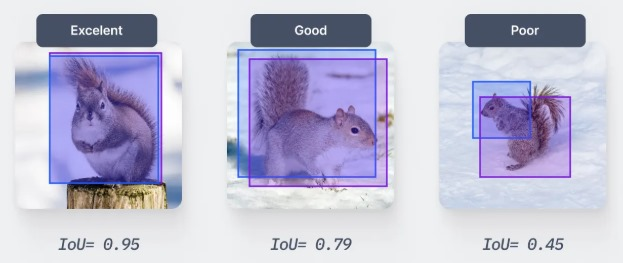
\includegraphics[scale=0.6]{gambar/bounding boc.jpg}
  % Keterangan gambar yang diinputkan
  \caption{Contoh perbandingan performa IoU }
  % Label referensi dari gambar yang diinputkan
  \label{fig:Perbandingan Intersection over Union }
\end{figure}
IoU menawarkan metode kuantitatif untuk mengevaluasi seberapa akurat model dalam
mengenali dan menandai objek dalam gambar. Dalam proses pelatihan, nilai IoU minimal yang
ditetapkan memungkinkan penetapan batas bagi kotak prediksi untuk dianggap cocok dengan
deteksi yang benar, memfasilitasi penyesuaian antara tingkat akurasi deteksi dan insiden false positif. Penentuan batas IoU tidak bersifat tetap dan dapat disesuaikan, dengan 0,5 yang menjadi standar patokan awal. Kotak prediksi dengan IoU minimal 0,5 terhadap deteksi positif dianggap valid. Penyesuaian ambang nilai ini mempengaruhi balance antara presisi dan daya tangkap, dengan peningkatan nilai ambang cenderung mengurangi kesalahan positif namun berpotensi mengabaikan beberapa deteksi valid.Penggunaan nilai kebenaran dasar dalam IoU merupakan perbandingan standar antara prediksi dan kondisi aktual objek yang diidentifikasi. Penandaan kotak kebenaran dasar, dilakukan secara manual oleh pakar, menentukan batas pasti objek dalam gambar. Skor IoU yang dihasilkan dari perbandingan antara prediksi model dengan batas ini memberikan wawasan terhadap efektivitas model dalam deteksi objek. Dataset kebenaran dasar, yang meliputi kotak pembatas yang ditandai secara manual, menjadi kunci dalam proses evaluasi ini, memberikan dasar objektif untuk mengukur kinerja algoritme deteksi objek\cite{Shah2023}.

\subsection{Tensorflow}
TensorFlow adalah sistem pembelajaran mesin yang beroperasi dalam skala besar dan di lingkungan yang heterogen. TensorFlow menggunakan grafik aliran data untuk merepresentasikan komputasi, status bersama, dan operasi yang mengubah status tersebut. Ini memetakan node grafik aliran data di banyak mesin dalam sebuah cluster, dan di dalam mesin di beberapa perangkat komputasi, termasuk CPU multicore, general-purpose GPU, dan ASIC yang dirancang khusus yang dikenal sebagai Tensor Processing Units (TPU). Arsitektur ini memberikan fleksibilitas kepada pengembang aplikasi. TensorFlow memungkinkan pengembang bereksperimen dengan pengoptimalan baru dan algoritma pelatihan. TensorFlow mendukung berbagai aplikasi, dengan dukungan yang sangat kuat untuk pelatihan dan inferensi pada jaringan neural dalam. Beberapa layanan Google menggunakan TensorFlow dalam produksinya, dan telah banyak digunakan untuk penelitian pembelajaran mesin.

\subsubsection{Tensorflow-Keras}
Keras merupakan library yang dikembangkan oleh Francois Chollet. Keras ini dirancang oleh pengembang agar cepat, mudah diimplementasikan, dan modular secara alami. Keras diadopsi sebagai API tingkat tinggi untuk mengembangkan algoritma pembelajaran mendalam alias deep learning. 


\subsection{Roboflow}
RoboFlow adalah platform yang mendukung pengembangan dan penyebaran aplikasi visi komputer dengan menyediakan fitur - fitur untuk manajemen dan peningkatan dataset. Platform ini dirancang untuk memudahkan pengolahan, analisis, dan augmentasi data visual, sehingga mempercepat siklus pengembangan dan peningkatan model pembelajaran mesin.

\begin{figure}[H]
  \centering

  % Ubah dengan nama file gambar dan ukuran yang akan digunakan
  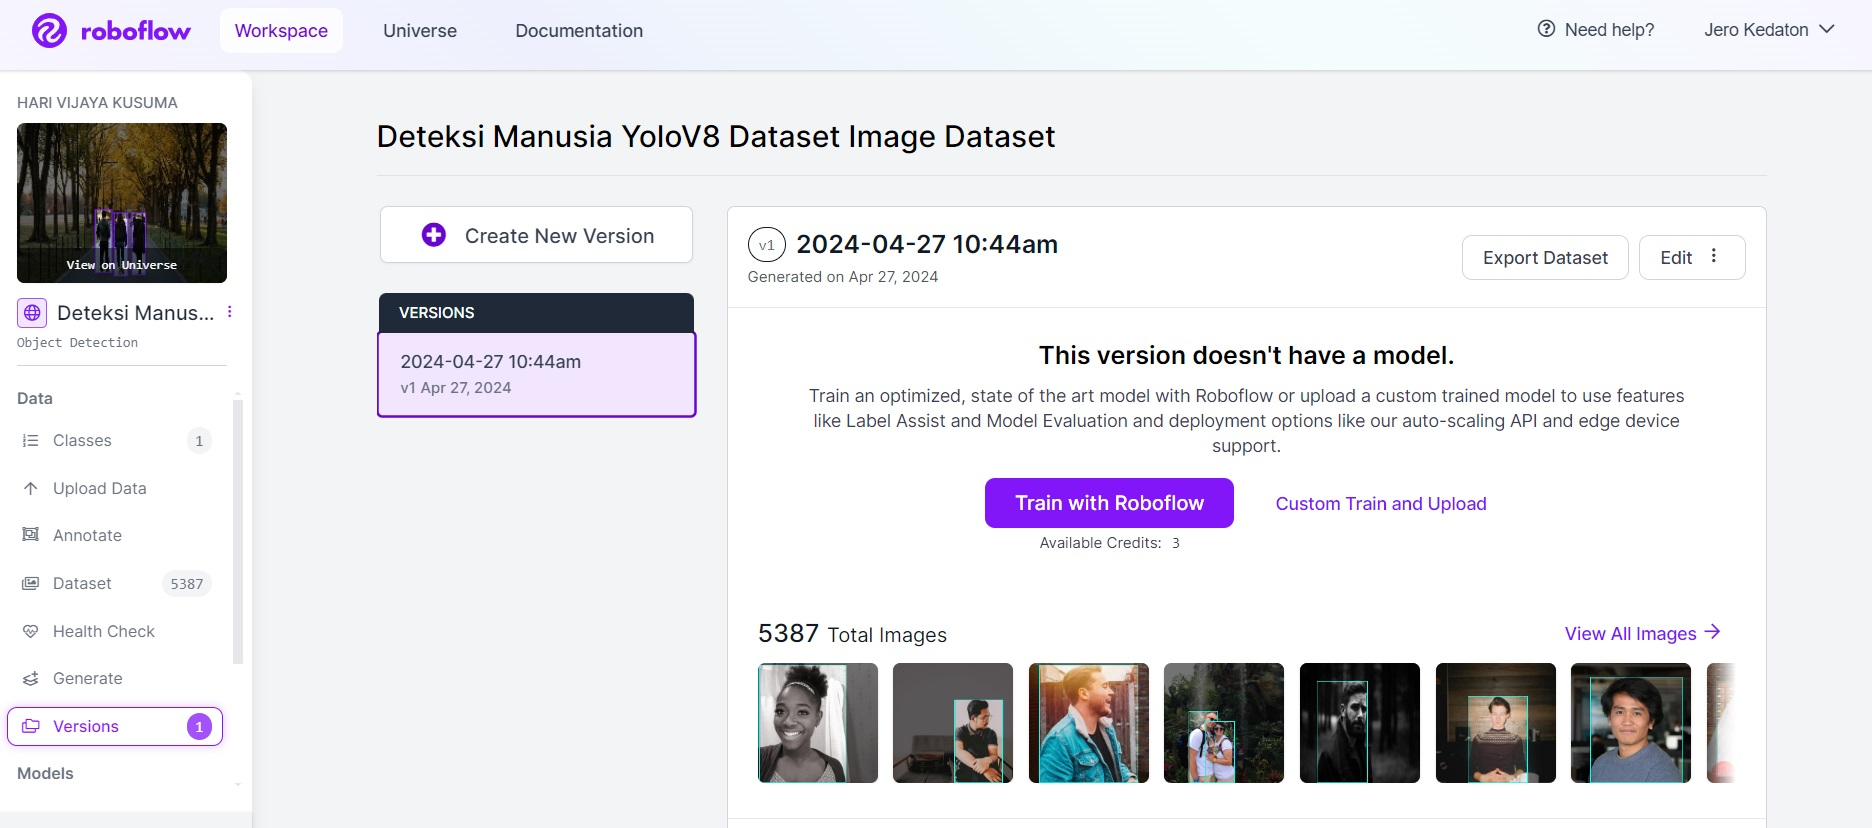
\includegraphics[scale=0.3]{gambar/roboflow.jpg}

  % Ubah dengan keterangan gambar yang diinginkan
  \caption{Interface Roboflow}
  \label{fig:roboflow}
\end{figure}

RoboFlow menyediakan serangkaian fungsi yang membantu dalam proses pengembangan model visi komputer, termasuk:
\begin{itemize}
    \item Annotasi Data : RoboFlow memungkinkan pengguna untuk menandai gambar dengan alat bantu yang intuitif, mempercepat proses pembuatan label untuk dataset.
    \item Augmentasi Data: Melalui augmentasi data, RoboFlow dapat secara otomatis memodifikasi gambar dalam dataset untuk menciptakan variasi, yang membantu dalam meni- ngkatkan robustness model yang dilatih.
    \item Konversi Format Data: Platform ini mendukung konversi antara berbagai format dataset yang populer, memudahkan pengguna dalam mempersiapkan data untuk berbagai jenis algoritma pembelajaran mesin.
    \item Pemisahan Dataset: RoboFlow menyediakan fungsi untuk membagi dataset menjadi set pelatihan, validasi, dan pengujian, yang merupakan langkah penting dalam validasi model.
\end{itemize}
RoboFlow menawarkan integrasi yang mulus dengan banyak kerangka kerja pembelajaran mesin populer seperti TensorFlow, PyTorch, dan YOLO. Integrasi ini memungkinkan pengembang:
\begin{itemize}
    \item Ekspor Data: Pengguna dapat dengan mudah mengekspor dataset mereka dalam format yang siap digunakan oleh kerangka kerja pembelajaran mesin pilihan mereka.
    \item Pelatihan Model: Platform ini menyediakan alat yang memungkinkan pengguna untuk langsung melatih model mereka menggunakan dataset yang telah disiapkan dan dioptimalkan.
    \item Evaluasi Model: RoboFlow menyediakan metrik untuk mengukur kinerja model, membantu pengguna memahami efektivitas model mereka dan membuat penyesuaian yang diperlukan.
\end{itemize}


\subsection{ESP-32}
ESP32 adalah modul mikrokontroler terintegrasi yang memiliki fitur lengkap dan kinerja tinggi. Modul ini merupakan pengembangan dari ESP8266, yang merupakan modul WiFi populer. ESP32 memiliki dua prosesor komputasi, satu prosesor untuk mengelola jaringan WiFi dan Bluetooth, serta satu prosesor lainnya untuk menjalankan aplikasi. Dilengkapi dengan memori RAM yang cukup besar untuk menyimpan data. Fitur yang berguna seperti TCP/IP, HTTP, dan FTP. Modul ini juga dilengkapi fitur pemrosesan sinyal analog, dukungan untuk sensor, dan dukungan untuk perangkat masukan/keluaran (I/O) digital. ESP32 juga memiliki dukungan untuk konektivitas Bluetooth. Dapat digunakan untuk mengendalikan perangkat yang terhubung dengan Bluetooth.